\chapter{Multiagent Problem Formulation}
\label{cha:problemfor}


The goal of multiagent systems' research is to find methods that allow
us to build complex systems composed of autonomous agents who, while
operating on local knowledge and possessing only limited abilities,
are nonetheless capable of enacting the desired global behaviors. We
want to know how to take a description of what a \emph{system of
  agents} should do and break it down into individual agent behaviors.
At its most ambitious, multiagent systems aims at reverse-engineering
emergent phenomena as typified by ant colonies, the economy, and the
immune system. Multiagent systems approaches the problem using the
well proven tools from game theory, Economics, and Biology. It
supplements these with ideas and algorithms from artificial
intelligence research, namely planning, reasoning methods, search
methods, and machine learning.

\mc{A more relaxed introduction to the topics in this chapter is given
  in \cite[Chapters 16--17]{russell03a}.} These disparate influences
have lead to the development of many different approaches, some of
which end up being incompatible with each other.  That is, it is
sometimes not clear if two researchers are studying variations of the
same problem or completely different problems.  Still, the model that
has thus far gained most attention, probably due to its flexibility as
well as its well established roots in game theory and artificial
intelligence, is that of modeling agents as utility maximizers who
inhabit some kind of Markov decision process.  This is the model we
present in this chapter and the one we will use most often throughout
the book. Note, however, that while this is a very general model it is
not always the best way to describe the problem.  We will also examine
the traditional artificial intelligence planning model and, in later
chapters, models inspired by Biology. Another popular model is that of
agents as logical inference machines. This model is favored by those
working on semantic or logical applications. We will sometimes make
reference to \td{deductive} agents which can deduce facts based on the
rules of logic, and \td{inductive} agents (see
Chapter~\ref{cha:learn-mult-syst}) which use machine learning
techniques to extrapolate conclusions from the given evidence.


\section{Utility}

A common simplifying assumption is that an agent's preferences are
captured by a \td{utility function}.  This function provides a map
from the states of the world or outcome of game to a real number.
\mc{In game theory it is known as the von Neumann-Morgenstern utility
  function.} The bigger the number the more the agent likes that
particular state.  Specifically, given that $S$ is the set of states
in the world the agent can perceive then agent $i$'s utility function
is of the form

\begin{equation}
  \label{eq:utility}
  u_i : S \rightarrow \Re.
\end{equation}

Notice also that the states are defined as those states of the world
that the agent can perceive. For example, if a robot has only one
sensor that feeds him a binary input, say 1 if it is bright and 0 if
its dark, then that robot has a utility function defined over only two
states regardless of how complicated the real world might be, such as
$u_i(0) = 5$, $u_i(1) = 10$. In practice, agents have sophisticated
inputs and it is impractical to define a different output for each
input. Thus, most agents also end up mapping their raw inputs to a
smaller set of world states. Creating this mapping function can be
challenging as it requires a deep understanding of the problem
setting.

Given an agent's utility function we can define a \td{preference
  ordering} for the agent over the states of the world.  By comparing
the utility values of two states we can determine which one is
preferred by the agent. This ordering has the following properties.
\begin{itemize}
\item \emph{reflexive}: $u_i(s) \geq u_i(s)$
  
\item \emph{transitive}: If $u_i(a) \geq u_i(b)$ and $u_i(b) \geq u_i(c)$ then $u_i(a) \geq u_i(c)$.
  
\item \emph{comparable}: $\forall_{a,b}$
  either $u_i(a) \geq u_i(b)$ or $u_i(b) \geq u_i(a)$. 
\end{itemize} 

We can use utility functions to describe the behavior of almost every
agent. Utility functions are also useful for capturing the various
tradeoffs that an agent must make, along with the value or expected
value of its actions. For example, we can say that a robot receives a
certain payment for delivering a package but also incurs a cost in
terms of the electricity used as well as the opportunity cost---he
could have been delivering other packages. If we translate all these
payments and costs into utility numbers then we can easily study the
tradeoffs among them.

Once we have defined a utility function for all the agents then all
they have to do is take actions which maximize their utility. As in
game theory, we use the word \td{selfish} to refer to a rational agent
that wants to maximize its utility. Notice that this use is slightly
different from the everyday usage of the word which often implies a
desire to harm others, a true selfish agent cares exclusively about
its utility. The use of selfish agents does not preclude the
implementation of cooperative multiagent systems.
\mc{\textbf{selfish}, adj.  Devoid of consideration for the
  selfishness of others. ---\emph{The Devil's Dictionary}}We can view
a cooperative multiagent system as one where the agents' utility
functions have been defined in such a way so that the agents seem to
cooperate. For example, if an agent receives a higher utility for
helping other agents then the resulting behavior will seem cooperative
to an observer even though the agent is acting selfishly.

We use utility functions as a succinct way of representing an agent's
behavior. In the actual implementations these functions will sometimes
be probabilistic, sometimes they will be learned as the agent acts in
the world, sometimes they will be incomplete, sometimes they will be
the result of some inferencing or induction. Still, by assuming that
the function exists we can more easily design and study a multiagent
system.


\subsection{Utility is Not Money}
\label{sec:money}

Note that while utility represents an agent's preferences it is not
necessarily equated with money. In fact, the utility of money has been
found to be roughly logarithmic. For example, say Bill has \$100
million while Tim has \$0 in the bank. They both contemplate the
possibility of winning one million dollars. Clearly, that extra
million will make a significant difference in Tim's lifestyle while
Bill's lifestyle will remain largely unchanged, thus Tim's utility for
the same million dollars is much larger than Bill's. There is
experimental evidence that shows most people have these type of
conditional preferences. Very roughly, people's utility for smaller
amounts of money is linear but for larger amounts it becomes
logarithmic. Notice that we are considering the \td{marginal utility}
of money, that is, it is the utility for the next million dollars.  We
assume that both Bill and Tim have the same utility for their first
million dollars.  \mc{You can determine your own curve by repeatedly
  asking yourself for increasing values of $x$: which one would you
  rather have, $x$ dollars, or a $50/50$ chance at winning $2\cdot x$
  dollars? When you start preferring the first choice you are dropping
  below the $y=x$ line.}

Recent results in behavioral economics have shown that the true
utility function is more complicated than what can be captured by a
mathematical function \cite{camerer03a}. One experiment shows that
people are less likely to take a gamble when the wording of the
question is such that the person must give back some money, even if
the gamble is mathematically identical to another one that uses
different wording. The experiment in question is the following: which
option would you prefer (a) I give you \$10,000 and a 50/50 chance at
winning another \$10,000, or (b) I give you \$20,000 and then flip a
coin and if it comes out heads you have to give me \$10,000. Both of
these are equivalent but a large majority of people prefer option (a).

The fact that people are not entirely rational when making choices
about money becomes important to us when we start to think about
building agents that will buy, sell, or negotiate for humans. It is
reasonable to assume that in these systems people will demand agents
that behave like people. Otherwise, the agent would be making
decisions the user finds disagreeable. People's apparent irrationality
also opens up the possibility that we could build agents that are
better negotiators than us.

\subsection{Expected Utility}
\label{sec:expected-utility}

Once we have utility functions we must then determine how the agents
will use them. We assume each agent has some sensors which it can use
to determine the state of the world and some effectors which it can
use to take action.  These actions can lead to new states of the
world. For example, an agent senses its location and decides to move
forward one foot. Of course, these sensors and effectors might not
operate perfectly: the agent might not move exactly one foot or its
sensors might be noisy. Let's assume, however, that the agent does
know the probability of reaching state $s'$ given that it is in state
$s$ and takes action $a$. This probability is given by $T(s,a,s')$
which we call the \td{transition function}. Since the transition
function returns a probability then it must be true that the sum of
$T(s,a,s')$ over all possible $a$ and $s'$ is equal to one.

Using this transition function the agent can then calculate its
\td{expected utility} for taking action $a$ in state $s$ as
\begin{equation}
  \label{eq:mod-eu}
  E[u_i,s,a] = \sum_{s' \in S} T(s,a,s')u_i(s'),
\end{equation}
where $S$ is the set of all possible states. 

An agent can use the expected utility function to determine the value
of a piece of added information it might acquire such as an extra
sensor reading or a message from another agent. For example, consider
a piece of new information that leads the agent to determine that it
is not really in state $s$ but it is instead in state $t$. Perhaps a
second agent tells him that he is near a precipice and not in the
middle of a plateau as the agent originally thought. In this case the
agent can compare the expected utility it would have received under
the old state against the new one it will now receive. That is, the
\td{value of information} for that piece of information is given by
\begin{equation}
  \label{eq:mod-valueinfo}
  E[u_i,t,\pi_i(t)] -  E[u_i,t,\pi_i(s)].
\end{equation}
The value of the piece of information is the expected utility the
agent receives now that he knows he is in $t$ and takes action
accordingly minus the utility it would have received if he had instead
mistakenly assumed it was in $s$ and taken action accordingly. This
equation provides a simple and robust way for agents to make
meta-level decisions about what knowledge to seek: what messages to
send, which sensors to turn on, how much deliberation to perform, etc.

Specifically, an agent can use it to play \emph{``what if''} games to
determine its best action in the same way a person might. For example,
say a doctor has made a preliminary decision about which drug to
prescribe for a patient but is uncertain about the patient's specific
disease. She can calculate the value of information acquired from
performing various tests which could identify the specific disease. If
a test, regardless of its outcome, would still lead the doctor to
prescribe the same drug then the value of the information from that
test's result is zero: it does not lead to a change in action so
\eqref{eq:mod-valueinfo} is zero. On the other hand, a test that is
likely to change the doctor's action will likely have a high value of
information.


\section{Markov Decision Processes}
\label{sec:mark-decis-proc}
\mpic{models/markov2}{Andrey Markov}{1856}{1922}{}


So far we have assumed that only the agent can change the state of the
world. But, the reality in most cases is that agents inhabit an
environment whose state changes either because of the agent's action
or due to some external event. We can think of the agent sensing the
state of the world then taking an action which leads it to a new
state. We also make the further simplifying assumption that the choice
of the new state therefore depends only on the agent's current state
and the agent's action. This idea is formally captured by a \td{Markov
  decision process} or \acro{mdp}.
\begin{definition}[Markov Decision Processess]
  An \acro{mdp} consists of an initial state $s_1$ taken from a set of
  states $S$, a transition function $T(s,a,s')$ and a reward function
  $r: S \rightarrow \Re$.
\end{definition}

The transition function $T(s,a,s')$ gives us the probability that an
agent in state $s$ who takes action $a$ will end up in state $s'$.
For a purely \td{deterministic} world we have that this function will
be zero for all $s'$ of each given $s,a$ pair except one, for which it
will be one.  That is, in a deterministic world an agent's action has
a completely predictable effect. This is not the case for a
\td{non-deterministic} environment where an agent's action could lead
to a number of different states, depending on the value of this fixed
probability function.

\begin{SCfigure}
  \begin{minipage}{1.0\linewidth}
    \begin{center}
      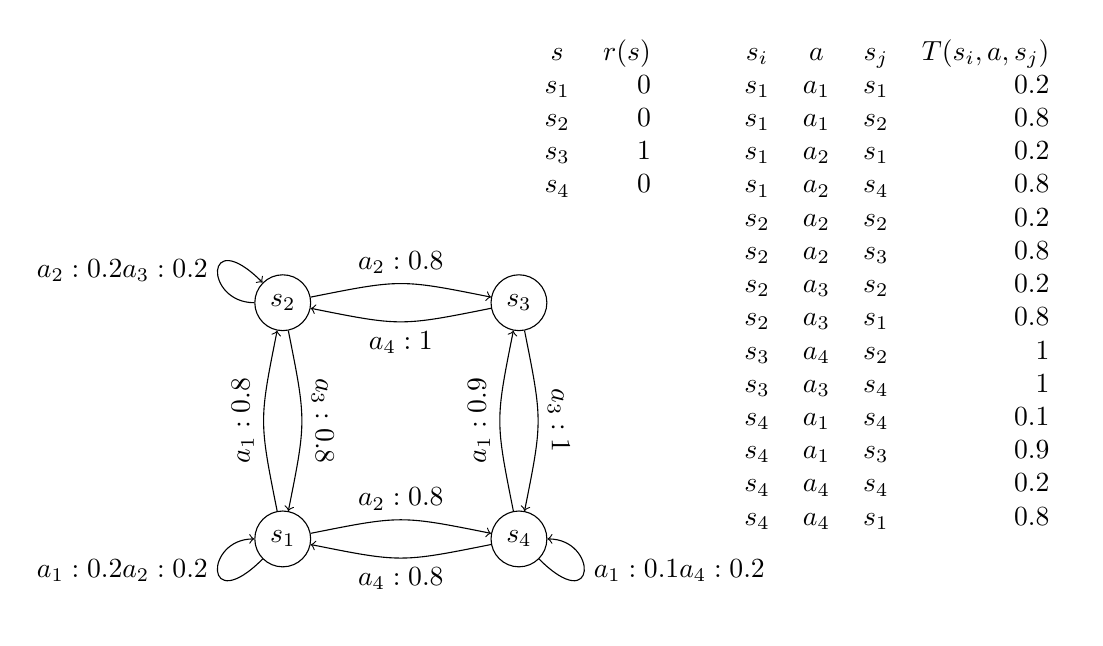
\begin{tikzpicture}
        \node[draw,circle] (s1) at (0,0) {$s_1$};
        \node[draw,circle] (s2) at (0,3) {$s_2$};
        \node[draw,circle] (s3) at (3,3) {$s_3$};
        \node[draw,circle] (s4) at (3,0) {$s_4$};
        \draw[->] (s1) .. controls (-.3,1.5)
        .. node[above,sloped] {$a_1: 0.8$} (s2);
        \draw[->] (s1) .. controls (-1,-1) and (-1,0) .. node[left]
        {\snugbox{$a_1 : 0.2$ \\$a_2 : 0.2$}} (s1);
        \draw[->] (s1) .. controls (1.5,.3) .. node[above,sloped]
        {$a_2 : 0.8$} (s4);
        \draw[->] (s2) .. controls (.3,1.5) .. node[above,sloped]
        {$a_3 : 0.8$} (s1);
        \draw[->] (s2) .. controls (1.5,3.3) .. node[above,sloped]
        {$a_2 : 0.8$} (s3);
        \draw[->] (s2) .. controls (-1,3) and (-1,4) .. node[left]
        {\snugbox{$a_2 : 0.2$ \\ $a_3 : 0.2$}} (s2);
        \draw[->] (s3) .. controls (1.5,2.7) .. node[below,sloped]
        {$a_4 : 1$} (s2);
        \draw[->] (s3) .. controls (3.3,1.5) .. node[above,sloped]
        {$a_3 : 1$} (s4);
        \draw[->] (s4) .. controls (2.7,1.5) ..
        node[above,sloped] {$a_1 : 0.9$} (s3);
       \draw[->] (s4) .. controls (4,-1) and (4,0) .. node[right]
       {\snugbox{$a_1 : 0.1$\\$a_4 : 0.2$}} (s4);
       \draw[->] (s4) .. controls (1.5,-.3) .. node[below,sloped]
       {$a_4: 0.8$} (s1);

        \node[below] (t) at (7.8,6.5)  {
          \begin{tabular}{cccr} \toprule
            $s_i$ & $a$ & $s_j$ & $T(s_i,a,s_j)$ \\ \midrule
            $s_1$ & $a_1$ & $s_1$ & $0.2$ \\
            $s_1$ & $a_1$ & $s_2$ & $0.8$ \\
            $s_1$ & $a_2$ & $s_1$ & $0.2$ \\
            $s_1$ & $a_2$ & $s_4$ & $0.8$ \\ 
            $s_2$ & $a_2$ & $s_2$ & $0.2$ \\
            $s_2$ & $a_2$ & $s_3$ & $0.8$ \\
            $s_2$ & $a_3$ & $s_2$ & $0.2$ \\
            $s_2$ & $a_3$ & $s_1$ & $0.8$ \\ 
            $s_3$ & $a_4$ & $s_2$ & $1$ \\
            $s_3$ & $a_3$ & $s_4$ & $1$ \\
            $s_4$ & $a_1$ & $s_4$ & $0.1$ \\
            $s_4$ & $a_1$ & $s_3$ & $0.9$ \\
            $s_4$ & $a_4$ & $s_4$ & $0.2$ \\
            $s_4$ & $a_4$ & $s_1$ & $0.8$ \\  \bottomrule
          \end{tabular}
        };
        \node[below] (r) at (4,6.5) {
          \begin{tabular}{cr} \toprule
            $s$ & $r(s)$ \\ \midrule
            $s_1$ & 0 \\
            $s_2$ & 0 \\
            $s_3$ & 1 \\
            $s_4$ & 0 \\ \bottomrule
          \end{tabular}
        };
      \end{tikzpicture}
    \end{center}
  \end{minipage}
  \caption{Graphical representation of a sample Markov decision
    process along with values for the transition and reward functions.
    We let the start state be $s_1$.}
  \label{fig:markovprocess}
\end{SCfigure}

Figure~\ref{fig:markovprocess} shows a typical visualization of an
\acro{mdp}, this one with four states. Notice that in this example the
agent's actions are limited based on the state, for example, in state
$s_1$ the agent can only take actions $a_1$ and $a_2$. Also note that
when the agent is in state $s_1$ and it takes action $a_1$ there is a
$0.2$ probability that it will stay in the same state. In this example
the agent receives a reward of 1 only when it reaches $s_3$, at which
point its only option is to leave $s_3$.

The agent's behavior is captured by a \td{policy} which is a mapping
from states to actions. We will use $\pi$ to denote the agent's
policy. The agent's goal then becomes that of finding its \td{optimal
  policy} which is the one that maximizes its expected utility, as we
might expect a selfish agent to do. This strategy is known as the
principle of \td{maximum expected utility}. Agent $i$'s optimal policy
can thus be defined as

\begin{equation}
  \label{eq:mod-meu}
  \pi^*_i(s) = \arg \max_{a \in A} E[u_i,s,a].
\end{equation}

But, in order to expand the expected value within that equation we
must first determine how to handle future rewards.  That is, is it
better to take 100 actions with no reward just to get to a state which
gives the agent a reward of 100, or is it better to take 100 actions
each of which gives the agent a reward of 1? Since no agent is likely
to live forever we will not want to wait forever for that big reward.
On the other hand, it seems reasonable to give up a small reward in
the next couple of steps if we know there is a very big reward
afterwards. As such, we generally prefer to use \td{discounted
  rewards} which allow us to smoothly reduce the impact of rewards
that are farther off in the future. We do this by multiplying the
agent's future rewards by an ever-decreasing \td{discount factor}
represented by $\gamma$, which is a number between zero and one.

For example, if an agent using policy $\pi$, starts out in state $s_1$
and visits states $s_1, s_2, s_3,\ldots$ then we say that its
discounted reward is given by
\begin{equation}
  \label{eq:mod-discounted}
  \gamma^0 r(s_1) + \gamma^1 r(s_2) + \gamma^2 r(s_3) + \cdots
\end{equation}
Note, however, that we only know $s_1$. The rest of the states, $s_2,
s_3,\ldots$ depend on the transition function $T$. That is, from state
$s_1$ we know that the probability of arriving at any other state $s'$
given that we took action $a$ is $T(s,a,s')$ but we do not know which
specific state the agent will reach. If we assume that the agent is an
utility maximizing agent then we know that it is going to take the
action which maximizes its expected utility. So, when in state $s$ the
agent will take action given by \eqref{eq:mod-meu}, which when
expanded using \eqref{eq:mod-eu} gives us 
\begin{equation}
  \label{eq:mod-bestaction}
  \pi^*(s) = \arg\max_a \sum_{s'} T(s,a,s') u(s'),
\end{equation}
\mpic{models/bellman}{Richard Bellman}{1920}{1984}{Norbert Wiener
  prize, IEEE Medal of Honor.}  where $u(s')$ is the utility the agent
can expect from reaching $s'$ and then continuing on to get more
rewards for successive states while using $\pi^*$.  We can now work
backwards and determine what is the value of $u(s)$. We know that when
the agent arrives in $s$ it receives a reward of $r(s)$, but we now
also know that because it is in $s$ it can take its action based on
$\pi^*(s)$ and will get a new reward at the next time.  Of course,
that reward will be discounted by $\gamma$.  As such, we can define
the real utility the agent receives for being in state $s$ as
\begin{equation}
  \label{eq:bellman}
  u(s) = r(s) + \gamma \max_a \sum_{s'} T(s,a,s')u(s').
\end{equation}
This is known as the \td{Bellman equation} and it captures the fact
that an agent's utility depends not only on its immediate rewards but
also on its future discounted rewards. Notice that, once we have this
function defined for all $s$ then we also have the agent's true
optimal policy $\pi^*(s)$, namely, the agent should take the action
which maximizes its expected utility, as given in
\eqref{eq:mod-bestaction}.

The problem we now face is how to calculate $u(s)$ given the
\acro{mdp} definition.  One approach is to solve the set of equations
formed. Given $n$ states we have $n$ Bellman equations each one with a
different variable. We thus have a system of $n$ equations with $n$
variables so, theoretically, we can find values for all these
variables. In practice, however, solving this set of equations is not
easy because of the $\max$ operator in the Bellman equation which
makes the equations non-linear.

\begin{SCfigure}
  \begin{minipage}{1.0\linewidth}
    \begin{codebox}
      \Procname{$\proc{value-iteration}(T,r,\gamma,\epsilon)$}
      \li \Do
      \li  $u \gets u'$
      \li $\delta \gets 0$
      \li \For $s \in S$ %foreach
      \li \Do $u'(s) \gets r(s) + \gamma \max_a \sum_{s'} T(s,a,s')
      u(s')$
      \li \If $|u'(s) - u(s)| > \delta$
      \li \Then $\delta \gets |u'(s) - u(s)|$
          \End
       \End
      \li \kw{until} $\delta < \epsilon(1-\gamma)/\gamma$
      \End
      \li \Return $u$
    \end{codebox}
  \end{minipage}
  \caption{The \proc{value-iteration} algorithm. It takes as input an
    \acro{mdp} given by $T(\cdot)$, a discount value $\gamma$, and an
    error $\epsilon$. It returns a $u(s)$ for that \acro{mdp} that is
    guaranteed to have an error less than $\epsilon$.}
  \label{fig:value-iter}
\end{SCfigure}

\begin{SCfigure}
  \begin{minipage}{1.0\linewidth}
  \begin{center}
  \begin{tabular}{lrrrrr} \toprule
             & \multicolumn{5}{c}{Time $(t)$} \\  \cmidrule{2-6} 
             & 0 & 1 & 2              & 3 & 4 \\ \midrule
    $u(s_1)$ & 0 & 0 & 0              & $.5(.8).45 = .18$ & $.5(.036 +
    .376) = .206$ \\
    $u(s_2)$ & 0 & 0 & $.5(.8)1 = .4$ & $.5(.88)1 = .44$ & $.5(.088 + .96) = .52$\\
    $u(s_3)$ & 0 & 1 & 1              &$1 + .5(1).45 = 1.2$ & $1 +
    .5(.47) = 1.2$ \\
    $u(s_4)$ & 0 & 0 & $.5(.9)1 =.45$ & $.5(.9 + .045) =.47$ & $.5(1.1 + .047) = .57$\\
    \bottomrule
  \end{tabular}

  \medskip

  \begin{tabular}{cc} \toprule
    $s$ & $\pi^*(s)$ \\ \midrule
    $s_1$ & $a_2$ \\
    $s_2$ & $a_2$ \\
    $s_3$ & $a_3$ \\
    $s_4$ & $a_1$ \\ \bottomrule
  \end{tabular}
  \end{center}
  \end{minipage}
  \caption{Example application of the \proc{value-iteration} algorithm
    to the MDP from figure~\ref{fig:markovprocess}, assuming
    $\gamma=.5$ and $\epsilon = .15$. The algorithm stops after $t=4$.
    The bottom table shows the optimal policy given the utility values
    found by the algorithm.}
  \label{fig:valueiterex}
\end{SCfigure}

Another approach for solving the problem is to use \td{value
  iteration}. In this method we start by setting the values of $u(s)$
to some arbitrary numbers and then iteratively improve these numbers
using the \td{Bellman update} equation:
\begin{equation}
  \label{eq:bellman-update}
  u^{t+1}(s) \gets r(s) + \gamma \max_a \sum_{s'}T(s,a,s')u^t(s').
\end{equation}
The reader will notice that this equation is nearly the same as
\eqref{eq:bellman}, except that we are now updating the $u$ values
over time. It has been shown that this process will eventually, and
often rapidly, converge to the real values of $u(s)$. We also know
that if the maximum change in utility for a particular time step is
less than $\epsilon(1-\gamma)/\gamma$ then the error is less than
$\epsilon$.  This fact can be used as a stopping condition.

\netlogo{valueiter}The \proc{value-iteration} algorithm is shown in
figure~\ref{fig:value-iter}. This algorithm is instance of \td{dynamic
  programming} in which the optimal solution to a problem is found by
first finding the optimal solutions to sub-problems. In our case, the
sub-problems are the variables themselves. Finding a value for one
variable helps us find values for other variables.

%In figure~\ref{fig:valueiterex} the top table shows how the utility
%values change over time. The bottom table shows the actions that a
%utility-maximizing agent would take given the utility values returned
%by the the algorithm.


For example, figure~\ref{fig:valueiterex} shows how the utility values
change as the \proc{value-iteration} algorithm is applied to the
example from figure~\ref{fig:markovprocess}. The utilities start at 0
but $s_3$ is quickly set to 1 because it receives a reward of 1.  This
reward then propagates back to its immediate neighbors $s_2$ and $s_4$
at time 2 and then at time 3 it reaches $s_1$. At time 4 the algorithm
stops because the biggest change in utility from time 3 to time 4 was
$0.13$, for $s_4$, which is less than or equal to
$\epsilon(1-\gamma)/\gamma = .15$.


\subsection{Multiagent Markov Decision Processes}
\label{sec:mult-mark-decis}

The \acro{mdp} model represents the problems of only one agent, not of
a multiagent system. There are several ways of transforming an
\acro{mdp} into a multiagent \acro{mdp}. The easiest way is to simply
place all the other agents' effects into the transition function. That
is, assume the other agents don't really exist as entities and are
merely part of the environment.  This technique can work for simple
cases where the agents are not changing their behavior since the
transition function in an \acro{mdp} must be fixed. Unfortunately,
agents that change their policies over time, either because of their
own learning or because of input from the users, are very common.

A better method is to extend the definition of \acro{mdp} to include
multiple agents all of which can take an action at each time step. As
such, instead of having a transition function $T(s,a,s')$ we have a
transition function $T(s,\va,s')$, where \va{} is a vector of size
equal to the number of agents where each element is an agent's action,
or a symbol representing non-action by that agent. We also need to
determine how the reward $r(s)$ is to be doled out amongst the agents.
One possibility is to divide it evenly among the agents.
Unfortunately, such a simplistic division can mislead agents by
rewarding them for bad actions. A better method is to give each agent
a reward proportional to his contribution to the system's reward. We
will see how this can be done in chapter~\ref{sec:coin}.

\subsection{Partially Observable MDPs}
\label{sec:part-observ-mdps}

In many situations it is not possible for the agent to sense the full
state of the world. Also, an agent's observations are often subject to
noise. For example, a robot has only limited sensors and might not be
able to see behind walls or hear soft sounds and its microphone might
sometimes fail to pick up sounds. For these scenarios we would like to
be able to describe the fact that the agent does not know in which
state it is in but, instead, believes that it can be in any number of
states with certain probability. For example, a robot might believe
that it is in any one of a number of rooms, each with equal
probability, but that it is definitely not outdoors. We can capture
this problem by modeling the agent's \td{belief state} \vb{} instead
of the world state. This belief state is merely a probability
distribution over the set of possible states and it indicates the
agent's belief that it is in that state.  For the case with four
states, the vector $\vb = \langle \frac{1}{2}, \frac{1}{2}, 0,
0\rangle$ indicates that the agent believes it is either in $s_1$ or
$s_2$, with equal probability, and that it is definitely not in $s_3$
or $s_4$.

We also need an \td{observation model} $O(s,o)$ which tells the agent
the probability that it will perceive observation $o$ when in state
$s$. The agent can then use the observations it receives to update its
current belief \vb{}. Specifically, if the agent's current belief is
\vb{} and it takes action $a$ then its new belief vector $\vb'$ can be
determined using
\begin{equation}
  \label{eq:pomdp-belief-update}
  \forall_{s'} \; \vb'(s') = \alpha O(s', o) \sum_s T(s,a,s')\, \vb(s),
\end{equation}
where $\vb(s)$ is the value of \vb{} for $s$ and $\alpha$ is a
normalizing constant that makes the belief state sum to 1. When we put
all these requirements together we have a \td{partially observable
  Markov decision process} or \acro{pomdp} which are a very natural
way of describing the problems faced by an agent with limited sensors.
Of course, since the agent does not know the state then it cannot use
value iteration to solve this problem.

Luckily, it turns out that we can use \eqref{eq:pomdp-belief-update}
to define a new transition function
\begin{equation}
  \label{eq:pomdp-transition}
  \tau(\vb,a,\vb') = \left\{ 
      \begin{array}{ll}
        \sum_{s'}O(s',o) \sum_s T(s,a,s')\,\vb(s) & \text{if
          \eqref{eq:pomdp-belief-update} is true for }\vb,a,\vb' \\
        0 & \text{otherwise,}
      \end{array}
      \right.
\end{equation}
and a new reward function
\begin{equation}
  \label{eq:pomdp-reward}
  \rho(\vb) = \sum_s \vb(s) r(s).
\end{equation}

Solving a \acro{pomdp} on a physical state amounts to solving this
\acro{mdp} on the belief state. Unfortunately, this \acro{mdp} can
have an infinite number of states since the beliefs are continuous
values. Luckily, there do exist algorithms for solving these type of
\acro{mdp}s. These algorithms work by grouping together beliefs into
regions and associating actions with each region. \mc{See
  \cite[Chapter 17.5]{russell03a} for introduction to dynamic decision
  networks.}In general, however, when faced with a \acro{pomdp}
problem it is usually easier to use a dynamic decision networks to
represent and solve the problem.


\section{Planning}
\label{sec:planning}

In the \td{artificial intelligence planning} problem an agent is also
given a set of possible states and is asked for a sequence of actions
that will lead it to a desirable world state. However, instead of a
transition function the agent is given a set of operators.  Each
operator has pre-requisites that specify when it can be used---in
which states---and effects which specify the changes the operator will
cause in the state. The planning problem is to find a sequence of
operators that take the agent from the start state to the goal state.

It should be clear that this problem is a special case of an
\acro{mdp}, one where only one state provides a reward and all the
transitions have probability of 1 or 0. The transitions are generated
by applying the operators to the current state. By describing the
problem using operators we achieve a much more succinct definition of
the problem than by enumerating all states and transition
probabilities as done in an \acro{mdp}. Still, our goal is solving the
problem, not defining it with as few bits as possible.  The more
detailed description of the states does, however, provide an advantage
over the simple state listing used in \acro{mdp}, namely, it provides
added information about the composition of the state. For example, if
we want to reach a state that has properties of \id{is-blue?} and
\id{is-wet?} then we can use this knowledge to set about getting the
state of the world blue and, once that is done, to get it wet without
changing its color. This kind of information is opaque in a \acro{mdp}
description which simply describes a wet blue state as $s_{11}$ and a
dry blue state as $s_{23}$. Operators and their corresponding state
descriptions thus provide the agent with more knowledge about the
problem domain.

There exists many planning algorithms which solve the basic planning
problem and variations of it, including cases where there is a
possibility that the operators don't have the desired effect (making
it even more like an \acro{mdp}), cases where the agent must start
taking actions before the plan can be finished, and cases where there
is uncertainty as to what state the agent is in (like \acro{pomdp}).
Most modern planning algorithms use a graphical representation of the
problem. That is, they end up turning the problem into an
\acro{mdp}-like problem and solving that.  These algorithms are
sophisticated and are available as libraries to use with your
programs. \mc{See \cite[Chapters 11--12]{russell03a} for pointers to
  these programs.}  If the need arises to solve a planning problem or
an \acro{mdp} it is advisable to use one of the many available
libraries or, at worst, implement one of the published algorithms
rather than trying to implement your own.


\subsection{Hierarchical Planning}
\label{sec:hier-plann}

A very successful technique for handling complexity is to recursively
divide a problem into smaller ones until we find problems that are
small enough that they can be solved in a reasonable amount of time.
This general idea is known as the \td{divide and conquer} approach in
\acro{ai}. Within planning, the idea can be applied by developing
plans whose primitive operators are other plans. For example, in order
to achieve your goal of a holiday at the beach you must first arrange
transportation, arrange lodging, and arrange meals. Each one of these
can be further decomposed into smaller actions, and there might be
different ways of performing this decomposition. Within the planning
model this amounts to building virtual operators which are planning
problems themselves, instead of atomic actions. The problem then
becomes one of deciding which virtual operators to build. In fact, the
problem is very similar to that of deciding which functions or classes
to write when implementing a large software project.

Within the \acro{mdp} model we can imagine building a hierarchy of policies,
each one taking of from states that fit a particular description (say,
dry states) to other types of states (say, red and wet). We can then
define new \acro{mdp} problems which use sets of states as atomic states and
the new policies as transition functions, similar to how we built
\acro{pomdp}s. These techniques are studied in \td{hierarchical learning}.

Hierarchical planning and learning are usually studied as ways of
making the planning and learning problems easier, that is, as ways to
develop algorithms that will find solutions faster. However, once
developed these hierarchies provide added benefits in a multiagent
system. Specifically, they can be used to enable coordination among
agents \cite{durfee99b}. By exchanging top-level plan names (or
policies) the agents have a general idea of what each other is doing
without the need for exchanging detailed instructions of what they are
doing at each step. For example, with two robots moving boxes in a
room one might tell the other that its moving a box from the South
corner to the East corner, the other agent then knows that if it stays
in the Northwest part of the room it does not need to worry about the
exact location of its partner---the robots stay out of each other's
way without detailed coordination. This technique of using
goal/plan/policy hierarchies for multiagent coordination has been very
successful. We will examine it in more detail in
Chapter~\ref{cha:hier-coord}.

\section{Summary}
\label{sec:summary}

The view of an autonomous agent as an utility-maximizing agent that
inhabits an \acro{mdp}, or variation thereof, is most popular because
of its flexibility, applicability to disparate domains, and
amenability to formal analysis with mathematical or computational
tools. As such, this book will largely adopt this model as the basis
for formulating the various multiagent problems. Note, however, that
the \acro{mdp} is a tool for describing the problem faced by an agent.
In practice, it is rare that a practical solution to a real world
problem is also implemented as an algorithm to solve the raw
\acro{mdp}. More commonly we find algorithms which use a much more
succinct, and therefore practical, method for representing the
problem. Unfortunately, these representations tend to be very domain
specific; they cannot be used in different domains.

\begin{exercises}
\item Marvin is a robot that inhabits a 3 by 3 grid and can only move
  North, South, East, and West. Marvin's wheels sometimes spin so that
  on each action there is a .2 probability that Marvin remains
  stationary. Marvin receives a reward of 1 whenever it visits the
  center square.
  \begin{enumerate}
  \item Draw an \acro{mdp} which describes Marvin's problem.
  \item What is the optimal policy?
  \end{enumerate}

\item The dynamic programming approach can be used to solve a wide
  variety of problems. For example, the Google search engine ranks
  results using the PageRank algorithm in which the pagerank of a
  webpage is proportional to the number of other pages that link to it
  weighted by their own pagerank. Thus, the pagerank can be calculated
  using a simple variation of the value iteration algorithm. However,
  one problem is that we do not know how long it will take for the
  algorithm to converge.

  Implement the \proc{value-iteration} algorithm from
  figure~\ref{fig:value-iter} and run experiments to determine how
  much time it takes to converge as you increase the number of states
  given a fixed edge to node ratio. Try different ratios.


\item You have a table with three blocks: A, B, C. Assume the state of
  the world is completely defined by the position of the blocks
  relative to each other, where a block can only be on the table on on
  top of another block. At most one block can be on top of another
  block block. You are further given the following operators:
  \begin{itemize}
  \item $\proc{move-to-table}(\id{block})$: Requires that \id{block}
    has no other block on top of it. Results in the block now being on
    the table.
  \item $\proc{move-to-block}(\id{b1}, \id{b2})$: Requires that block
    \id{b2} not have any other block on top of it. Results in block
    \id{b1} being on top of block \id{b2}.
  \end{itemize}
  Draw an \acro{mdp} for this domain assuming operators always have
  their intended results.


\item Implement a NetLogo program where the patches are randomly set
  to one of three colors: black, red, and green.There is a turtle in
  this world who can only move North, South, East, and West by one
  patch at a time. Each time it lands in a patch it receives a reward
  determined by the color of the patch: black is 0, red is -1, and
  green in 1.

  The turtle's movement is noisy, so when it decides to move North it
  ends up at the desired North tile with probability .5, and the tile
  NorthEast of its current location (a diagonally adjacent tile) with
  probability .25, and at the tile NorthWest of its current location
  with a probability of .25.

  Implement the \proc{value-iter} algorithm for this domain and find
  the optimal policy.
\end{exercises}



%The agent E:sensors -> agent -> action:E
%agent - knowledge base -< inference

%%% Local Variables: 
%%% mode: latex
%%% TeX-command-default: "PDFlatex"
%%% TeX-master: "~/wp/mas/mas"
%%% End: 

